%% %%%%%%%%%%%%%%%%%%%%%%%%%%%%%%%%%%%%%%%%%%%%%%%%%
%% Template for a conference paper, prepared for the
%% Food and Resource Economics Department - IFAS
%% UNIVERSITY OF FLORIDA
%% %%%%%%%%%%%%%%%%%%%%%%%%%%%%%%%%%%%%%%%%%%%%%%%%%
%% Version 1.0 // November 2019
%% %%%%%%%%%%%%%%%%%%%%%%%%%%%%%%%%%%%%%%%%%%%%%%%%%
%% Ariel Soto-Caro
%%  - asotocaro@ufl.edu
%%  - arielsotocaro@gmail.com
%% %%%%%%%%%%%%%%%%%%%%%%%%%%%%%%%%%%%%%%%%%%%%%%%%%
\documentclass[11pt]{article}
\usepackage{UF_FRED_paper_style}

\usepackage{lipsum}  %% Package to create dummy text (comment or erase before start)

%% ===============================================
%% Setting the line spacing (3 options: only pick one)
% \doublespacing
% \singlespacing
\onehalfspacing
%% ===============================================

\setlength{\droptitle}{-5em} %% Don't touch

% %%%%%%%%%%%%%%%%%%%%%%%%%%%%%%%%%%%%%%%%%%%%%%%%%%%%%%%%%%
% SET THE TITLE
% %%%%%%%%%%%%%%%%%%%%%%%%%%%%%%%%%%%%%%%%%%%%%%%%%%%%%%%%%%

% TITLE:
\title{Bayesian calibration of AeroModule code using DanAero data
% \thanks{Selected Paper prepared for presentation at the 201X Agricultural \& Applied Economics Association Annual Meeting}
}

% AUTHORS:
\author{Vinit Dighe\\% Name author
    \href{mailto:vinit@cwi.nl}{\texttt{vinit@cwi.nl}} %% Email author 1 
\and Benjamin Sanderse\\% Name author
    \href{mailto:b.sanderse@cwi.nl}{\texttt{b.sanderse@cwi.nl}} %% Email author 2
% \and Third Author\\% Name author
%     \href{mailto:thirdauthor@ufl.edu}{\texttt{thirdauthor@ufl.edu}}%% Email author 3
%\and Forth Author\\% Name author
%    \href{mailto:forthuthor@ufl.edu}{\texttt{forthuthor@ufl.edu}}%% Email author 4
    }
    
% DATE:
\date{\today}

% %%%%%%%%%%%%%%%%%%%%%%%%%%%%%%%%%%%%%%%%%%%%%%%%%%%%%%%%%%
% %%%%%%%%%%%%%%%%%%%%%%%%%%%%%%%%%%%%%%%%%%%%%%%%%%%%%%%%%%
\begin{document}
% %%%%%%%%%%%%%%%%%%%%%%%%%%%%%%%%%%%%%%%%%%%%%%%%%%%%%%%%%%
% %%%%%%%%%%%%%%%%%%%%%%%%%%%%%%%%%%%%%%%%%%%%%%%%%%%%%%%%%%
% ABSTRACT
% %%%%%%%%%%%%%%%%%%%%%%%%%%%%%%%%%%%%%%%%%%%%%%%%%%%%%%%%%%
% %%%%%%%%%%%%%%%%%%%%%%%%%%%%%%%%%%%%%%%%%%%%%%%%%%%%%%%%%%
{\setstretch{.8}
\maketitle
% %%%%%%%%%%%%%%%%%%
\begin{abstract}
% CONTENT OF ABS HERE--------------------------------------

\noindent A Bayesian framework using UQLab has been applied to calibrate the 3D correction factor used in the  axial force model implemented in the AeroModule code.   %% Dummy text for abstract. Erase before use.

% END CONTENT ABS------------------------------------------
\noindent
% \textit{\textbf{Keywords: }%
% key1; key2; key3; key4.} \\ %% <-- Keywords HERE!
% \noindent
% \textit{\textbf{JEL Classification: }%
% Q12; C22; D81.} %% <-- JEL code HERE!

\end{abstract}
}

% %%%%%%%%%%%%%%%%%%%%%%%%%%%%%%%%%%%%%%%%%%%%%%%%%%%%%%%%%%
% %%%%%%%%%%%%%%%%%%%%%%%%%%%%%%%%%%%%%%%%%%%%%%%%%%%%%%%%%%
% BODY OF THE DOCUMENT
% %%%%%%%%%%%%%%%%%%%%%%%%%%%%%%%%%%%%%%%%%%%%%%%%%%%%%%%%%%
% %%%%%%%%%%%%%%%%%%%%%%%%%%%%%%%%%%%%%%%%%%%%%%%%%%%%%%%%%%

% --------------------
\section{Introduction}


The wind energy industry is experiencing remarkable growths annually. Despite the great progress made, further cost reductions in wind turbine technology are necessary for wind energy to reach its full potential in terms of the large‐scale supply of electricity. Improving the reliability of aerodynamic models embedded in the design software currently used in industry is indispensable to guarantee reductions in the cost of wind energy.

Due to its relatively high computational efficiency compared to free‐wake vortex methods and CFD, the Blade‐Element‐Momentum (BEM) theory still forms the basis for many aerodynamic models. Yet various experimental campaigns have demonstrated that BEM‐based design codes are not always sufficiently reliable for predicting the aerodynamic load distributions on the wind turbine blades \citep{UAE_exp}. In many situations, the reliability of such codes was found to be unacceptable, in particular when comparing the predicted results by different aerodynamics/aeroelastic codes from various universities/institutions with the measurement data obtained from the UAE experimental campaigns. In some cases, deviations of the BEM predictions from the measurements exceeded 200\%, even though the simplest operating conditions of a wind turbine were being considered (i.e. uniform wind-speed and constant rotor speed, blade pitch and yaw angle). 

Wind tunnel tests on model turbines are indispensable to have a better understanding of the underlying physics and to improve engineering models for design codes. The controlled environment offered by a wind tunnel provides a set of measurements that is free from the uncertainties caused by the different atmospheric effects that are always present in open field tests of turbines. To improve the predictions of BEM‐based design codes, more reliable airfoil data models and inflow correction models are required. However, using the experimental data to improve these models is not an easy task. Two major problems are encountered: Firstly, measurement data is usually rare and limited. Secondly, there is a difficulty in determining accurately the angle of attack for the operating turbine.

In this investigation, we describe an approach for combining
observations from DanAero field experiments with predictions obtained using the TNO’s AeroModule aeroelastic (BEM) code  to carry out statistical
inference. Of particular interest here is determining uncertainty in the resulting predictions. This typically involves calibration of parameters in the computer model in response to the sensitivity analysis study carried by \citet{torque2020}.

In recent times, there has been increasing efforts in using Bayesian approach for the calibration of computer models. This is because of its ability to quantify uncertainties in input parameters while at the
same time reducing discrepancies between simulation
output and physical measurements. In the Bayesian
calibration of computer models, Markov Chain
Monte Carlo (MCMC) methods are a common way
for sampling from the posterior distributions of the
calibration parameters. Its widespread use can be
attributed to its ease of use in a wide variety of
problems. 


\section{DanAero experiment}

\begin{figure}
\centering
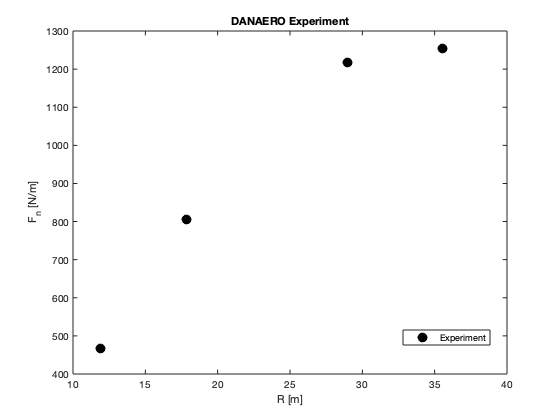
\includegraphics[width=0.65\textwidth]{exp.png}
\caption{Experimental blade forces denoting the mean normal forces along the blade radius $R$}
\label{pt1}
\end{figure}



A measurement campaign was carried out as part of the DanAero MW experiment \citep{DanAero}. A 2.3MW NM80 turbine located at the Tjæreborg Enge site and a nearby met mast were both instrumented with various sensors. ScaniValve system was used for the surface pressure measurements on the turbine blade. 


Besides the data obtained directly from the Tjæreborg Enge site,  a number of wind tunnel tests on different airfoils of NM80 turbine were also carried out in different wind tunnels \citep{tunnel}. The objective of the wind tunnel tests was to measure the lift, drag, moment, normal force coefficient and tangential force coefficient at four blade sections (13m, 19m, 30m, and 37m) of the LM38.8 blade (38.8m) which were instrumented with pressure taps.

The Tjæreborg experiment  database contains 35 Hz measurements and 10 minute statistics (mean, minimum, maximum and standard deviation) of all the data acquired by the DaqWin system as well as down sampled surface pressure measurements from five selected pressure taps at each of the four blade sections. All the data from the  experiments are available in data files with formats as explained in \citep{DanAero,tunnel}




\section{BEM model - AeroModule}

The aeroelastic BEM code - AeroModule  is used to model the aerodynamic and aeroelastic behaviour of wind turbine blades by combining the concept of momentum conservation of the flow (aerodynamic analysis) with the equations
of motion (structural analysis). In this work, we focus on the first aspect, namely the prediction of aerodynamic blade forces as given by the BEM method. For the purpose of calibration, normal aerodynamic forces (mean values) measured under non-sheared and non-yawed inflow conditions  has been selected from the measurements as described in \citep{DanAero}. The normal aerodynamic force on the blade surface is  calculated based on the following equation:

\begin{equation}
    F_n = 0.5\rho W^{2}c({{}{C}_l}_{3D} sin\beta + {{}{C}_d}_{3D} cos\beta),
\label{eq1}
\end{equation}

\noindent where $\rho$ is the fluid density, $W$ is the relative flow angle, $c$ is the chord length and $\beta$ is the relative flow angle. The 3D correction factor \citep{snel} has been applied to account for the effects of rotation on the lift and drag coefficients ($C_l$ and $C_d$). Then, the lift coefficient in equation \ref{eq1}  takes the following form:

\begin{equation}
    {{}{C}_l}_{3D} = 3.1(\frac{c}{r})^2(\frac{\Omega r}{W})^2({{}{C}_l}_{pot} - {{}{C}_l}_{2D})
\end{equation}

\noindent where $c$ is the local chord, $r$ is the local radius, $\Omega$ is the rotational speed of the rotor, ${{}{C}_l}_{pot}$ is the potential flow lift coefficient and ${{}{C}_l}_{2D}$ is the 2D lift coefficient. 

\section{Sensitivity analysis}

Before calibrating the BEM model, sensitivity analysis was performed to identify the parameters that have the most influence over the model’s output ($F_n$). The objective is to reduce the number of calibration parameters and choose only important parameters in the calibration process. This not only reduces computation cost but also
helps mitigate over-fitting. \citet{torque2020} observed that the model's output is basically only sensitive to the lift coefficient $C_l$ at the outward blade sections.

\begin{figure}
\centering
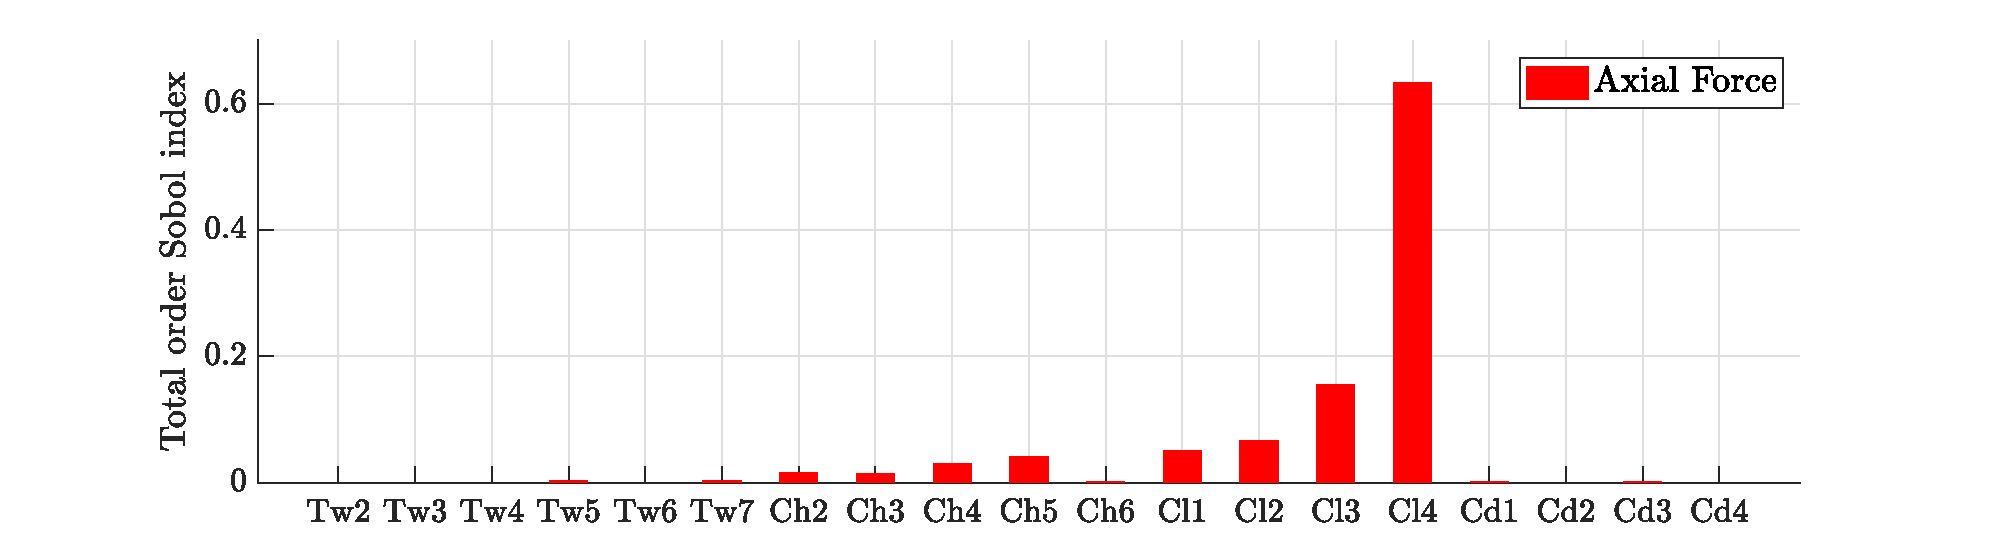
\includegraphics[width=0.70\textwidth]{ Sobol.pdf}
\label{pt1}
\caption{Sensitivity of axial force towards geometric and model uncertainties.}
\end{figure}

\section{Lift coefficient parametrization}

\citet{snel} derived a so-called `3D correction’ method  that gives an increase of the aerodynamic lift coefficient for the effects of rotation. The 3D factor 3.1 was originally used to fit with the DanAero measurements. Following the comparison of the UAE rotor experiment with the BEM code predictions, \citet{UAE_exp}  concluded that this factor could
as well be reduced to 3. Because it is
known that the term $(\frac{c}{r})^2$ is an empirical fit which gives a stronger dependency on $(\frac{c}{r})$ than
what is found from theory, it was decided to calibrate the the  3D factor; viz. a constant value for the range of $\alpha$ considered. Assuming a constant value of k, the $C_l$ curve at point 4 is  parametrized:

\begin{equation}
    {{}{C}_l}_{3D} = k(\alpha)(3.1 \pm \Delta)
    \label{eq3}
\end{equation}

\noindent where $k$ = $(\frac{c}{r})^2(\frac{\Omega r}{W})^2({{}{C}_l}_{pot} - {{}{C}_l}_{2D})$ as a function of angle of attack $\alpha$. 

\begin{figure}
\centering
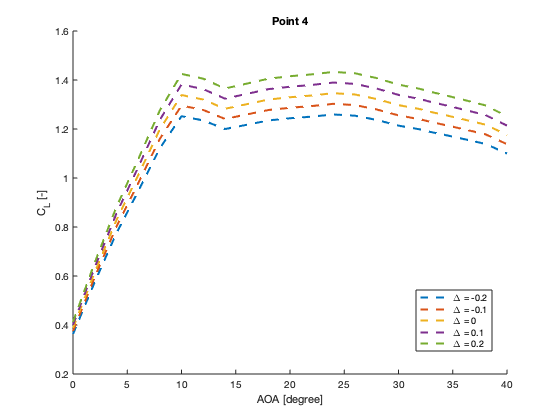
\includegraphics[width=0.65\textwidth]{ snel.png}
\label{pt1}
\caption{Realization of lift polar at point 4 using uniform distribution of $\Delta$}
\end{figure}




\section{Bayesian calibration}

Bayesian methods are used to estimate model parameter $\theta$  by combining two sources of information: prior information about $\theta$ and observations $D$ on output variables $x$. The prior information of $\theta$ is based on expert knowledge, literature review or by measuring parameters directly in the field or laboratory. In our case, $D$  as a function of $x$ are field measurements from the DanAero experiment. Bayes theorem makes it possible to combine the two
sources of information in order to calibrate $\theta$. The first step is to assign a probability distribution to $\theta$, representing our prior uncertainty about the value. In our case, we specified lower and upper bounds of the $\theta$'s uncertainty, defining the prior parameter distributions as uniform. The aim of Bayesian calibration is to reduce this uncertainty by using the $D$, thereby producing the posterior distribution for $\theta$. This is achieved by multiplying the prior with the likelihood function, which is the
probability of the $D$ given the $\theta$. The likelihood function is determined by the probability distribution of errors in
observations. To generate a representative sample of $\theta$ from the posterior distribution, we used  Markov Chain Monte Carlo (MCMC) methods.

\begin{center}
\begin{tabular}{ |c|c| } 
 \hline
 Symbol & Description  \\ 
 \hline
$D$ & Axial force at corresponding radial locations   \\ 
 $x$ & Angle of attack  \\ 
 $\theta$ & 3D factor\\
 \hline
\end{tabular}
\end{center}

\subsection{Metropolis-Hastings algorithm}


In the Metropolis–Hastings (MH) algorithm, a chain is initialized at a certain seed point $\theta^{(0)}$  belonging to an admissible domain. At iteration $t$ from the current point $x^{(t)}$, the algorithm randomly draws a new `candidate' parameter:

    \begin{equation*}
        \theta^{(*)} = \theta^{(t)} + \delta
    \end{equation*}
    \noindent where $\delta$ is a random vector generated from an uniform distribution on the interval (3.0,  3.2).
    
    Subsequently, the candidate is accepted with probability, if:
    
    \begin{equation*}
        \alpha = min \bigg\{1, \frac{p(\theta^{(*)}|D)}{p(\theta^{(t)}|D)}\bigg\},
    \end{equation*}
    
    % \begin{equation*}
    %     a = \frac{p(\theta^{*}|D)}{p(\theta_{t}|D)} = \frac{p(D|\theta^{*}) p(\theta^{*})}{p(D|\theta_{i-1})p(\theta_{i-1})}
    % \end{equation*}
    
    \noindent and rejected otherwise. It is important to note that the model evidence term cancels out from the acceptance probability. This avoids the calculation of the often intractable
integral. The candidate point $\theta^{(*)}$ is always accepted if its posterior value is no lower than the posterior value of $\theta^{(t-1)}$. Once the chain has attained the
N iterations, the chain must have converged to the target distribution
which is the posterior $\theta$ distribution.

\subsection{Adaptive Metropolis algorithm}

The basic idea of Adaptive Metropolis (AM) algorithm is to update the proposal distribution $p(\theta^{(*)}|D)$ by using the knowledge  acquired about the target distribution. Otherwise the definition of the AM algorithm is identical to the MH algorithm.

Suppose, therefore, that at time t we have sampled the states $x_{0}$, $x_{1}$, . . . , $x_{t}$, where $x_{0}$ is the initial state. Then, the posterior probability of the new 'candidate' parameter $\theta^{*}$ is accepted:

\begin{equation*}
        \alpha = min \bigg\{1, \frac{p(\theta^{(*)}|D)}{p(\theta^{(t)}|D)}\bigg\}, otherwise 
    \end{equation*}

\noindent where the proposal distribution $p(\theta^{(*)}|D)$ employed in AM algorithm is a Gaussian distribution with mean at the current point $\theta^{(t)}$ and covariance $C^{(t)}$ = $C^{(t)}$($x_{0}$, $x_{1}$, . . . , $x_{t}$). The AM algorithm is particularly useful over MH algorithm when a large number of samples from the same distribution is necessary (Bayesian calibration), and in CPU intensive applications, for example, optimization problems.


\subsection{Affine invariant ensemble algorithm}

MH and AM algorithm perform poorly when the target (i.e., posterior) distribution shows
strong correlation between the parameters. The performance of these algorithms can typically only be improved by considerable amount of tuning. The affine invariant ensemble algorithm (AIES)  reduces this problem. AIES algorithm has the property of being invariant to affine transformations to the target distribution. This means that if there exists an affine transformation of the difficult-to-sample
(by standard MCMC methods) target distribution to an easier-to-sample target distribution,
AIES samples both distributions equally easily without explicitly requiring this affine transformation.

The affine invariance property is achieved by generating proposals according to a so-called stretch move. This refers to proposing the new 'candidate' parameter by:

\begin{equation*}
    \theta^{*} = \theta^{(t)} + Z \hspace{1cm} where \hspace{1cm} Z \sim p(z) = \begin{cases}
    \frac{1}{\sqrt{z}(2\sqrt{a}-\frac{2}{\sqrt{a}})},& \text{if } z \epsilon [\frac{1}{a},a],\\
    0,              & \text{otherwise}.
\end{cases}
\end{equation*}

\noindent This requires sampling from the distribution $p(z)$ defined by the tuning parameter $a$, which is often set to $a$ = 2. The
candidate $\theta^{(*)}$ is then accepted with probability:


\begin{equation*}
        \alpha = min \bigg\{1, z^{M-1} \frac{p(\theta^{(*)}|D)}{p(\theta^{(t)}|D)}\bigg\},
    \end{equation*}

\noindent where $M$ is a scaled identity matrix. A practical advantage of the AIES algorithm is that it only has a single scalar tuning parameter $a$, and on the other hand, due to
its sequential nature, the algorithm cannot be parallelized which makes it comparably slower in comparison to the MH and AM algorithms.

\section{Results and discussion}
\begin{figure}
\centering
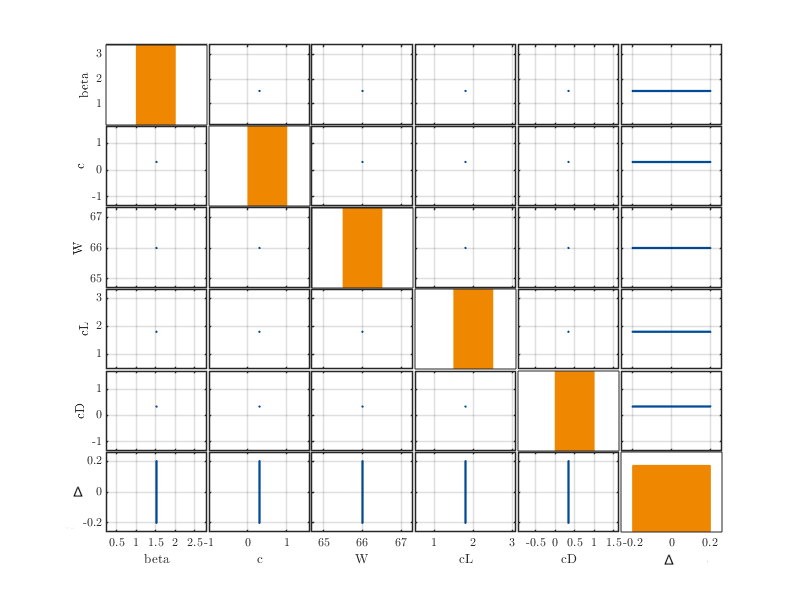
\includegraphics[width=0.7\textwidth]{prior.png}
\caption{Prior distribution of the parameters used in the axial force model.}
\label{prior}
\end{figure}

The information from the AeroModule run was utilised
to construct the prior distributions shown in Figure \ref{prior}. We compare the effectiveness of three MCMC algorithms: MH, AM and AIES. The comparison was carried out using the following metrics:

\begin{itemize}
    \item Trace plots: Trace plots are plots of the Markov chains versus the sample steps and can be useful for assessing convergence. As chains are typically initialized at random points,  the distribution of points can give valuable insights about convergence. 
    \item Gelman-Rubin diagnostics (\^{R}): A quantitative approach to assess convergence was introduced by  \citet{gelman}. \^{R} is the ratio of
between independent chain variance to  the combination of all chain variance
and is based on the concept that if multiple
chains have converged, there should be little variability between independent and the combination of all chains. For convergence, \^{R} should be approximately 1 $\pm$ 0.1. 
\end{itemize}

For comparison, the same number of iterations were run for all three algorithms. The first 50\% samples are discarded as burn-in to reduce the influence of the starting values.

\begin{figure}[htp]

\centering
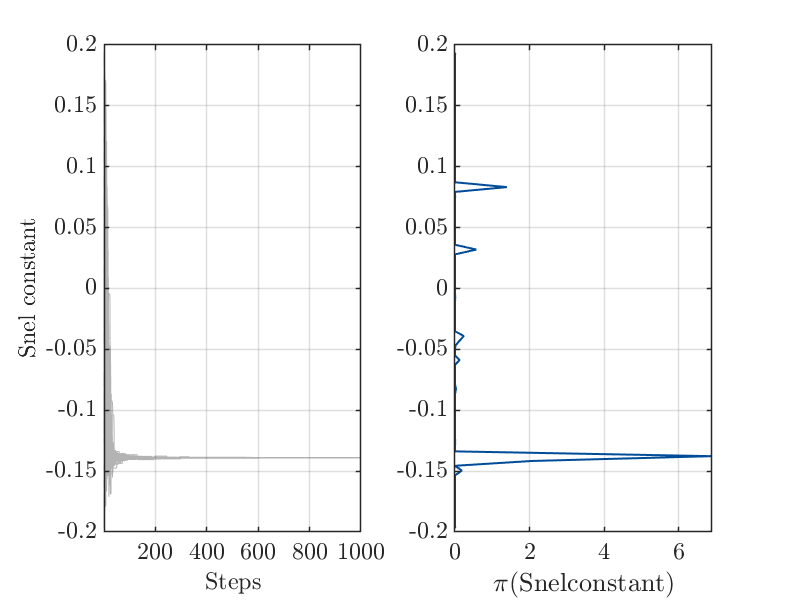
\includegraphics[width=.3\textwidth]{ trace_mh.png}\hfill
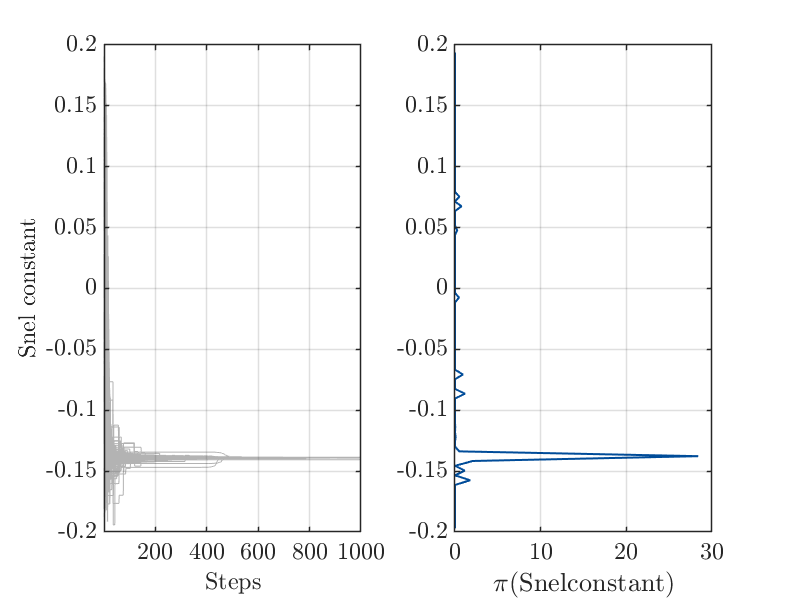
\includegraphics[width=.3\textwidth]{ trace_am.png}\hfill
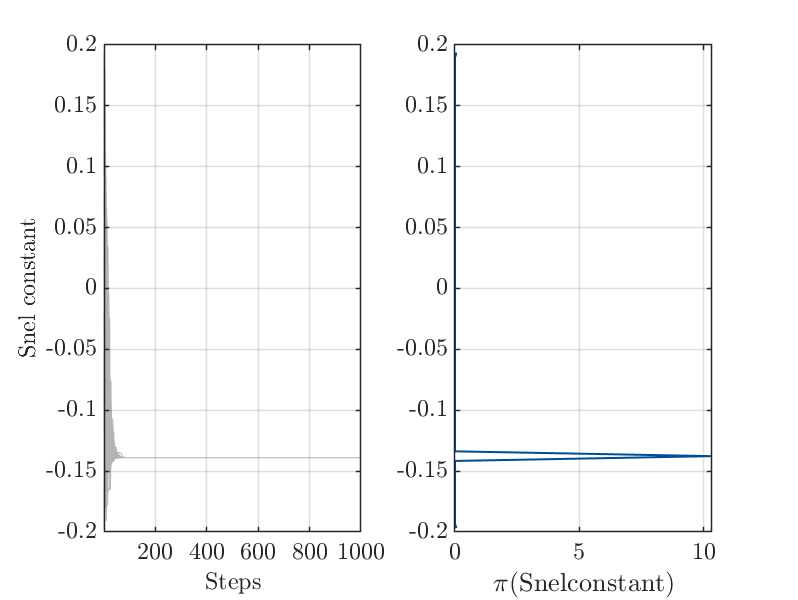
\includegraphics[width=.3\textwidth]{ trace.png}

\caption{Trace plots for the same number of iterations obtained with MH (left), AM (center) and AIES (right) algorithms.}
\label{trace}

\end{figure}


\begin{figure}
\centering
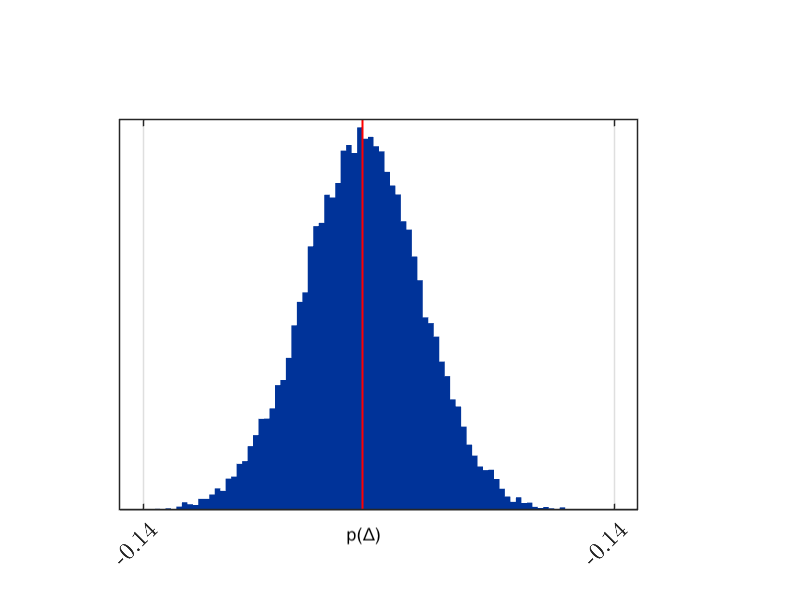
\includegraphics[width=0.45\textwidth]{ post1.png}
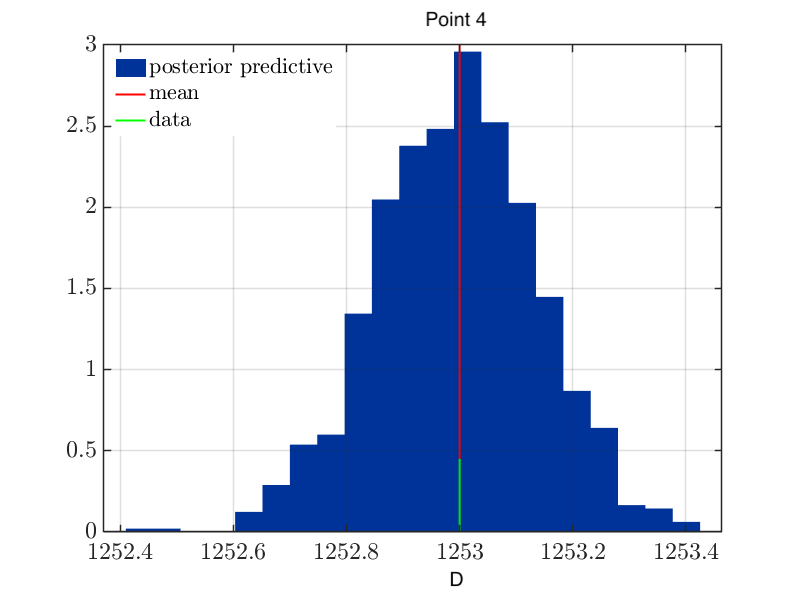
\includegraphics[width=0.45\textwidth]{ y1.png}
\caption{Posterior distribution of $\delta$ (left) along with posterior distribution of $D$ (right).}
\label{post}
\end{figure}



Figure \ref{trace}  provides a visual comparison of
the trace plots (including burn-in)
with samples generated by the three different MCMC algorithms. MH and AM algorithms demonstrate
bad mixing for the calibration parameters $\theta$, indicating that the algorithm does not sufficiently
explore the parameter space. After 1000 iterations
the calibration parameters for MH and AM algorithms have \^{R} = 2.276 \& 5.96 respectively. AIES algorithm performs
better, with the calibration parameters $\theta$ achieving
adequate convergence (\^{R} = 1.04) after 1000 iterations.
Trace plot (Figure \ref{trace} (right)) also shows good mixing. As with the AIES algorithm, the posterior distribution for $\Delta$ is plotted in Figure \ref{post}. Then, as in equation \ref{eq3}, the calibrated  $\theta$ = 3.1 - 0.14 = 2.96. 


\section{Conclusions}
Bayesian calibration framework using UQLab was tested using the DanAero data (axial force meaurement) to calibrate the 3D factor used in the AeroModule code. The governing forward model (axial force model) was obtained. This is followed by using the existing sensitivity analysis study to reduce the number of calibration parameters. The effectiveness of three MCMC algorithms (MH, AM and AIES) were
evaluated. Following the Bayesian calibration, the calibrated forward model suggests the 3D factor value equal to 2.96.
\medskip

\bibliography{references.bib} 



\end{document}